\documentclass[9pt,t]{beamer}
\usetheme{Wisconsin}
\usepackage[utf8]{inputenc}
\setbeamertemplate{page number in head/foot}[totalframenumber]
\setbeamerfont{block body}{size=\footnotesize}
\setbeamerfont{author}{size=\LARGE}
\setbeamerfont{date}{size=\Large}
\setlength{\leftmargini}{0pt}

%subcaptions
\usepackage{subcaption}
% \captionsetup[subfigure]{labelformat=empty} % turn off labeling figures

% turn off Figure in captions
\usepackage{caption}
% \captionsetup[figure]{labelformat=empty}

\newcommand{\QOR}{\qquad \text{OR} \qquad}
\newcommand{\QAND}{\qquad \text{AND} \qquad}
\newcommand{\QTHUS}{\qquad \text{THUS} \qquad}
\newcommand{\QTHEN}{\qquad \text{THEN} \qquad}
\newcommand{\QWITH}{\qquad \text{WITH} \qquad}
\newcommand{\QFOR}{\qquad \text{FOR} \qquad}
\newcommand{\QSO}{\qquad \text{SO} \qquad}
\newcommand{\QWHERE}{\qquad \text{WHERE} \qquad}
\newcommand{\LINE}{\par\noindent\rule{\textwidth}{0.4pt}\par}
\newcommand{\toinf}{\rightarrow\infty}
\newcommand{\tozero}{\rightarrow0}
\newcommand{\qeq}{\overset{?}{=}}
\newcommand{\ceq}{\overset{\checkmark}{=}}
\renewcommand{\epsilon}{\varepsilon}


% Roman Numerals
\newcommand{\rom}[1]{\expandafter\uppercase{\Romannumeral #1\relax}}

% hypersetup
\usepackage{hyperref}
\hypersetup{colorlinks,
            linkcolor = white,
            citecolor = white,
            urlcolor = cyan
}


\def\brac#1{\{#1\}}
\def\Brac#1{\big\{#1\big\}}
\def\BRAC#1{\bigg\{#1\bigg\}}
\def\angbrac#1{\langle#1\rangle}
\def\Angbrac#1{\big\langle#1\big\rangle}
\def\ANGBRAC#1{\bigg\langle#1\bigg\rangle}

% % Transitional slides between sections
% \AtBeginSection[]
% {
%     \begin{frame}
%         \frametitle{Table of Contents}
%         \tableofcontents[currentsection]
%     \end{frame}
% }


% Bibliography
\usepackage[sorting=none]{biblatex} %Imports biblatex package and cites in order of appearance
\addbibresource{mc2023_pres.bib} %Import the bibliography file
% make all font colors white
\setbeamercolor{bibliography item}{fg=white}
\setbeamercolor{bibliography entry author}{fg=white}
\setbeamercolor{bibliography entry title}{fg=white}
\setbeamercolor{bibliography entry location}{fg=white}
\setbeamercolor{bibliography entry note}{fg=white}
% adds numeric labels linked to bib entries
\setbeamertemplate{bibliography item}{\insertbiblabel}

% eliminate header within an environment
\makeatletter
    \newenvironment{withoutheadline}{
       \setbeamertemplate{headline}[default]
       \def\beamer@entrycode{\vspace*{-\headheight}}
    }{}
\makeatother

\title{Verification of the Cardinal Multiphysics Solver}
\subtitle{1-D Coupled Heat Transfer and Neutron Transport}
\author{Lewis Gross\vspace*{-1cm}}
\date{August 15, 2022}
%%----------------------------------------------------------------------------%%
\begin{document}

\begin{withoutheadline}
\begin{frame}[plain] % the plain makes the first frame look good
    \maketitle
\end{frame}
\end{withoutheadline}

%%----------------------------------------------------------------------------%%
%% Overview
%%----------------------------------------------------------------------------%%
\begin{withoutheadline}
\begin{frame}{Outline}
  \tableofcontents
\end{frame}
\end{withoutheadline}


%%----------------------------------------------------------------------------%%
%% Section 1
%%----------------------------------------------------------------------------%%
\section{Introduction}
\begin{frame}{Introduction}
    \begin{itemize}
        \item Multiphysics simulation
        \item Wide amount of codes (mention a few)
        \item Cardinal - our software choices
        \item Importance of V\&V, trustworthiness
        \item Verification via analytical benchmarks
    \end{itemize}
\end{frame}


%%----------------------------------------------------------------------------%%
%% Section 2
%%----------------------------------------------------------------------------%%
\section{Analytical Benchmark}
\begin{frame}{Analytical Benchmark}
    \begin{itemize}
        \item Greisheimer and Kooreman 1D coupled heat transfer and neutron transport \cite{analytical-benchmark}
        \item Describe physics, quantities and system
        \begin{equation}
                NEUTRON
        \end{equation}
        \begin{equation}
                HEAT
        \end{equation}
        \item where $\lambda \equiv (\frac{1}{k_{eff}}\frac{\nu \Sigma_{f}}{\Sigma_{t}} + \frac{\Sigma_{s}}{\Sigma_{t}} )$ is 
        the combined inscattering and quasistatic fission source term \cite{analytical-benchmark}, $q$ is the energy released
        \textbf{per reaction}
    \end{itemize}
\end{frame}

\begin{frame}{System Domain, Differential Equations, and Boundary conditions}
    \begin{itemize}
        \item Assumptions
        \begin{itemize}
            \item $S_{2}$ transport (i.e. $\mu=\pm 1$)
            \item Doppler-broadening
            \begin{equation}
                \sigma_{t}(x) = \sigma_{t,0}\sqrt{\frac{T_{0}}{T(x)}}.
            \end{equation}
            \item 1D thermal expansion
            \begin{equation} \label{sec:intro:density}
                \rho(x) =  \rho_{0} \sqrt{\frac{T_{0}}{T(x)}}.
            \end{equation}
            \item The fundamental assumption that yields an analytical solution: $T(x)=f\phi(x)$. Implies condition for HTC and $\sigma_{t,0}$
        \end{itemize}
    \end{itemize}
\end{frame}

\begin{frame}{System Domain, Differential Equations, and Boundary conditions}
    \begin{figure}[H]
        \centering
        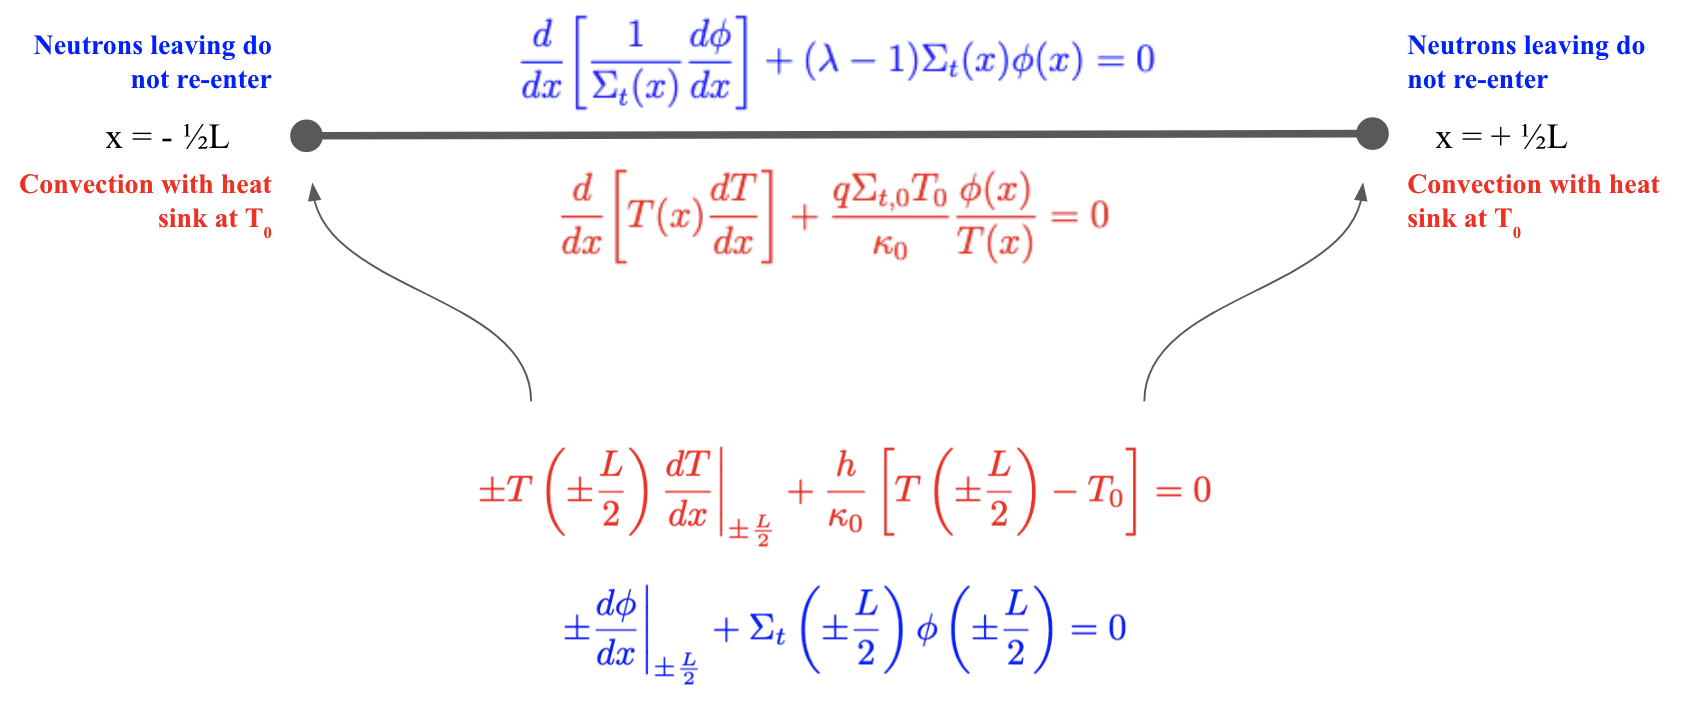
\includegraphics[width=0.95\linewidth]{figures/1D_Benchmark_Diagram.png}
    \end{figure}
    \begin{itemize}
        \item Analytical solution
        \begin{equation}
            \phi(x) = \phi(0) \sqrt{1 - \frac{(\lambda - 1)P^{2}x^{2}}{L^{2}q^{2}\phi^2(0)}}
        \end{equation}
    \end{itemize}
\end{frame}
%%----------------------------------------------------------------------------%%
%% Section 3
%%----------------------------------------------------------------------------%%
\section{Computational Model}
\begin{frame}{OpenMC Model}
    \begin{itemize}
        \item
    \end{itemize}
\end{frame}

\begin{frame}{MOOSE Heat Conduction Model}
    \begin{itemize}
        \item
    \end{itemize}
\end{frame}

\begin{frame}{Coupling, Data Mapping, and Convergence Criteria}
    \begin{itemize}
        \item
    \end{itemize}
\end{frame}


%%----------------------------------------------------------------------------%%
%% Section 4
%%----------------------------------------------------------------------------%%
\section{Results and Discussion}
\begin{frame}{Outputs and Comparisons}
    \begin{itemize}
        \item results
    \end{itemize}
\end{frame}

\begin{frame}{Future and companion work}
    \begin{itemize}
        \item discuss
    \end{itemize}
\end{frame}

%%----------------------------------------------------------------------------%%
%% Bibliography
%%----------------------------------------------------------------------------%%

\begin{frame}{Cite Dump}
    \begin{itemize}
        \item \cite{aya2023} \cite{brown-entropy-2006} \cite{dufek} \cite{lindsay2022moose} \cite{nekrs} \cite{novak-2023} \cite{novak2022-cardinal} \cite{openmc}
    \end{itemize}
\end{frame}

\begin{frame}[allowframebreaks]{Bibliography}
    \printbibliography
\end{frame}

\begin{frame}{Asides}
    \begin{itemize}
        \item Going from the Transport Equation to the ODE that describes neutron transport for this benchmark
        \item 
    \end{itemize}
\end{frame}


\end{document}
